%authentication
\section{Authentication}
We have chosen to implement a social media sign-in option because it does not require us to handle the user's passwords and other personal information. With a social media sign-in implemented in our application as a way of identifying the user, we move the security measures to the specific social media.
There are many different social media sign-in options such as Google+, Facebook, Twitter etc. We chose Google+ to be the first social media sign-in to implement. Other sign-in options could later be implemented in the application. It should be noted that it is not necessary for the user to be signed in to search for recipes, but actions like favouriting, adding to items to the shopping list, requires them to be signed in.

It makes sense to use Google+ sign-in since Google recommends Android users to have a Google account, because otherwise the user would limit their experience with an Android device. 
The Google+ sign-in authenticates the user and manages the OAuth 2.0 flow, which simplifies the integration with the Google \ac{api}s.
The Google+ sign-in process can seamlessly authenticate a user without them having to enter a password or even an account name. 
Once granted access the application is able to access to user's Google+ information through their Google+ account\cite{googleplusvideo}.

In the implementation of the Google+ sign-in we use an object called \\\inline{GoogleApiClient}\citep{googleapiclient-docs}, which is provided by the Google Play services application. 
The object \inline{GoogleApiClient} should be initialised and connected separately in every activity, so each activity has its own life cycle with the \inline{GoogleApiClient}, \autoref{fig:googleclientlifecycle} shows the basic life cycle of a \inline{GoogleApiClient} object in an activity.
\begin{figure}[H]
\centering
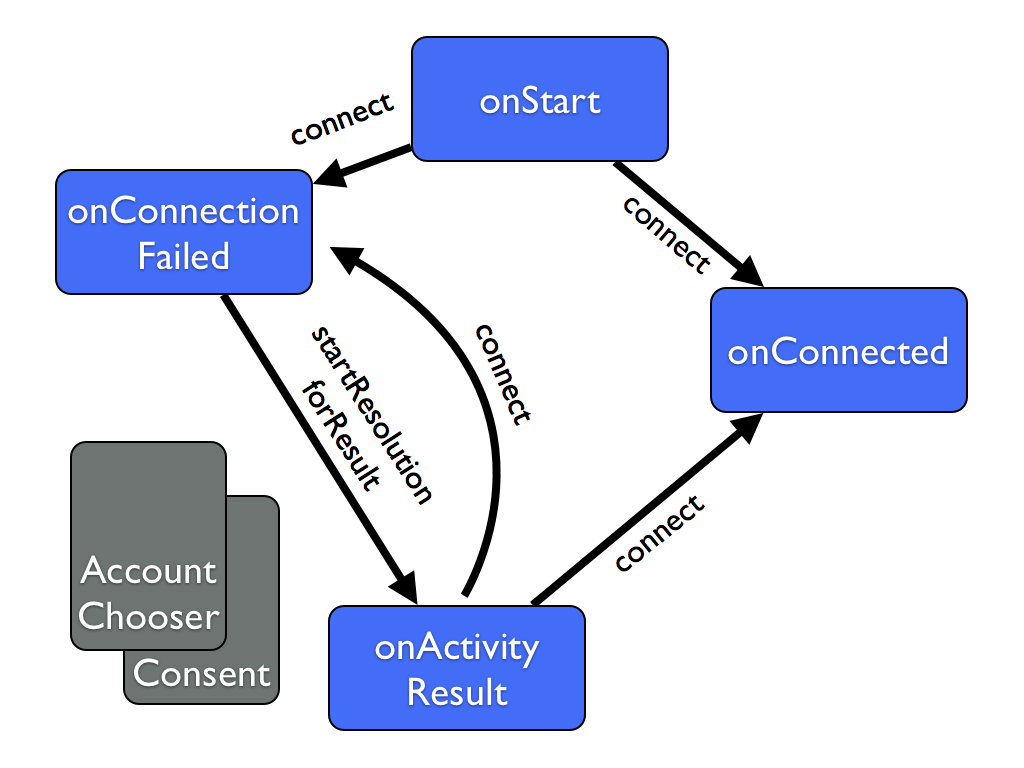
\includegraphics[width=0.75\linewidth]{img/googleclientflow.png}
\caption{The \inline{GoogleApiClient} basic life cycle\cite{googleapiclient-lifecycle}.}
\label{fig:googleclientlifecycle}
\end{figure}
We have implemented an activity called LogInActivity, which implements the sign-in features. Every activity in the application extends this activity, which means that all activities in the application has the sign-in feature. 
The blue boxes represents methods in the LogInActivity, and the two grey boxes represents other activities. The method \inline{onStart()} is invoked at activity start up, and we immediately try to sign-in. 
This can either succeed or fail, if it fails \inline{onConnectionFailed()} will be called, this will happen if the user has not yet consented with the Google+ sign-in, the application now awaits for them to press the sign-in button. 
When the user presses the sign-in button and they have multiple Google accounts, the application opens an account chooser activity.
After selecting the account that the user want to use, a consent activity will show presenting them with the Google+ information that the application should be allowed to access. 
When the user has granted the application access, then the result of the consent activity is returned to \inline{onActivityResult()}, and the user is signed in. 
If the user did not grant access to the application the routine starts all over. When the user is connected \inline{onConnected()} is called, this method simply updates the UI and downloads information from the user's Google+.

When the user is signed in to our application we can gain information of the user by using the \inline{GoogleApiClient}.
In our application we only use the user's Google email(account name) and their real name(for comments on recipes). 
When we receive the user's email we hash it using the SHA-256 hashing algorithm. We hash it because we have no use of the email other than its uniqueness, and from a security aspect it does not make sense to store their email in plain text both in the application and database. 
Every time the user makes an action that requires them to be signed in, we send their hashed email to the server together with the action. 
%It might seem redundant to send the hashed email every time and not just a user ID, but getting the user ID from the server turns out to be quite stressful to the server. Each time a user switches activity i.e. each time they view a recipe, the application signs in the user, and thus query the server for the user ID. Therefore it is more efficient just to send the hashed email with each user action.



